\chapter{Digital Surface Curvature}
\label{chap:estimators}

\begin{Abstract}
The surface curvature of continuous smooth lines and surfaces is a well-defined property, however, when working with point set data, mesh surfaces or 3D digital images, line and surface curvatures can only be estimated \cite{Kalogerakis_2007_RSEC} \cite{Klette_2004_DG} \cite{Mitra_2003_ESN}. In this chapter we review the nature of digitized surfaces and present a number of curvature estimators, two of which (the 3-cut mean estimator and the similarity curvature estimator) are new.\\
\end{Abstract}

%---------------- section ----------------
\section{Digitized Surfaces}

Digitized surfaces arise in numerous practical applications and the form that the digitization takes is highly application dependant. For a range of different applications, see, for example, \cite{Ikeuchi_2003_GBP}, \cite{Allen_2002_ABD}, \cite{Levoy_2000_TDMP}, \cite{Bloomenthal_1985_MMM}, and \cite{Roger_1980_BSS}. The data acquisition methods associated with surface digitization can be separated into two categories: volume-based and range-based. Consider, for example, the surface of a spherical object as illustrated in Figure~\ref{fig:estimators-digitize}(a).\\

Voxel digitizations, as shown, for example, in Figure~\ref{fig:estimators-digitize}(b), are volume-based, with the resultant data-set often being built up from multiple 2D scan slice layers. In volumetric applications, surfaces are usually defined as the boundary associated with a physical density discontinuity within an otherwise solid object (e.g. the medical application of locating bone surface within the volume of an arm). The voxel grid is usually regular, but the voxels are not necessarily cubes. This situation can arise, for example, from the fact that it is not uncommon for the distance between scan slices to be greater than the resolution within each 2D scan. Voxels are inherently volume elements, and as such, can only estimate actual surface location. See, for example, \cite{Sramek_1994_FSRRD} and \cite{Gargantini_1993_RMS}. However, it could be reasonably expected that each voxel would intersect the actual surface. Because voxel data is associated with positions in a fixed grid structure, a voxel data-set can be stored as integers which index position within that grid.\\

For examples of techniques which employ volumetric data structures, see \cite{Fournier_2006_3DDT} and\cite{Montani_1990_RVD}.  For a comprehensive theoretical treatment of voxel digitization that draws on concepts from topology, see \cite{Kovalevsky_2008_GLFS} and \cite{Kovalevsky_2003_MCL3M}.\\

%+++++++++++++++++++++++++++++++++++++++++
\begin{figure}[!t]
\begin{center}
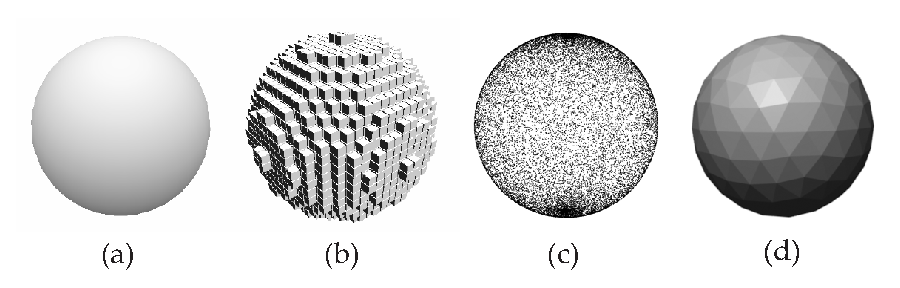
\epsfig{file=chapters/Estimators/digitize, width=125mm}
\end{center}
\caption{(a) Sphere surface. (b) Voxel digitization. (c) Point cloud digitization. (d) Triangle mesh digitization.}
\label{fig:estimators-digitize}
\end{figure}
%+++++++++++++++++++++++++++++++++++++++++

Point cloud digitizations are range-based (e.g., laser triangulation or laser 
time-of-flight) and the data consists of 3D space points, presented possibly in no 
particular sequence, and generally with unequal point separation distance. In 
Figure~\ref{fig:estimators-digitize}(c), for example, the concentration of points is 
greater at the top and bottom poles of the sphere. Unlike a voxel digitization, each point 
in a point cloud digitization is considered (ideally) to lie on the actual surface. Point 
cloud data is usually stored as a collection of real number 3D space coordinates.\\

For a curvature estimation technique that works directly with point cloud data as input, 
see \cite{Tong_2005_REATC}. Their work builds on previous work in which the concept of 
\emph{tensor voting} is developed \cite{Tang_1999_EGETV}. For an approach in which the 
local surface geometry in point cloud data is modeled by a set of quadratic curves see 
\cite{Agam_2005_ASFACE}, \cite{Agam_2005_APDE} and \cite{Tang_2004_CBLSG}.\\

Triangle mesh digitizations, as shown, for example, in 
Figure~\ref{fig:estimators-digitize}(d), approximate an actual surface as a set of 
adjoining flat triangular surface patches. It seems reasonable to assume that at least some 
part of each triangle patch would intersect the actual surface, but, in practice, there is 
no specific general rule. The triangle mesh data structure is often thought of as 
consisting of \emph{points}, \emph{edges} and \emph{faces}. The face adjacency pattern is 
an essential characteristic of a triangle mesh, and this adjacency is exploited by many 
triangle mesh processing algorithms.\\

Triangle meshes are the standard data structure used in 3D graphics modeling; see, for example, \cite{Foley_1996_CGPP}. 3D graphics modeling is a very active research area resulting in varied and numerous techniques. See, for example, books \cite{Lengyel_2004_M3DGP} and \cite{Hill_2007_CGOG}. Triangle meshes can be derived from both voxel based and point cloud digitizations (e.g. \cite{Cooper_2003_AMS3D}, \cite{Kobbelt_2001_FSSE}, \cite{Curless_2000_FRS3D}, \cite{Curless_1996_VMBCM}), and in this sense can be thought of as having higher order structure. Alternatively, a triangle mesh can also arise naturally when a range scan is acquired using a controlled rasterization pattern.\\

Most real-world digitization processes introduce noticeable \emph{noise} into the acquired 
data-set. This noise results in some uncertainty as to wether or not, for example, a voxel 
actually intersects the real surface, or a point in a point cloud actually lies on the real 
surface. Fortunately, it is possible to mathematically model noise and to reduce its 
negative impact through \emph{filtering}(e.g. \cite{Rugis_2006_ESC}, \cite{Rugis_2006_SRMRSD}).

Henceforth, we will refer to the data-set associated with a surface digitization as a \emph{digital surface}.\\

%---------------- section ----------------
\section{Gaussian and Mean Curvature Estimators}
All of the curvature estimators presented in this chapter require known point adjacency 
neighborhood information. This adjacency information is inherent in a triangle 
mesh\footnote{For any given set of surface points, more than one triangulation is possible, 
however, this does not affect the validity of the curvature estimators which are 
presented.} and, for convenience, we limit our consideration to triangle meshes. In 
practice, this restriction to triangle meshes is not particularly limiting in that 
conversion from other digitization types is usually possible.\\

The estimators used in this book are all \emph{local} in the sense that only knowledge of 
the nearby neighboring points is used in the computation of curvature.\\

%------------- subsection ----------------
\subsection{Triangle Umbrella}
\label{sec:estimators-umbrella}
First we review existing Gaussian and mean curvature estimators used by other authors, for example, \cite{Alboul_1996_PMSR}, \cite{Dyn_2000_OTUDCA}, and \cite{Meek_2000_SNGC}, which rely on knowledge of a complete \emph{triangle umbrela} neighborhood around a point of interest.\\

\begin{figure}[!t]
\begin{center}
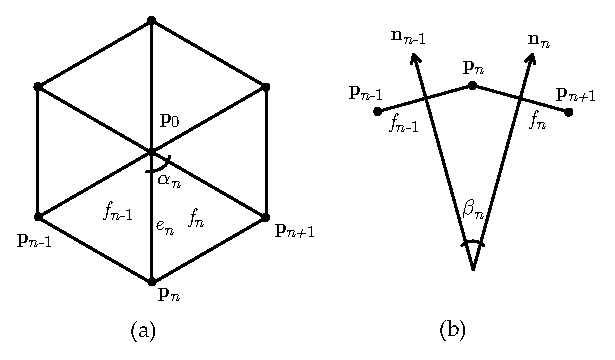
\epsfig{file=chapters/Estimators/estimators5, width=100mm}
\end{center}
\vspace{-10pt}
\caption{Triangle fan surface patch: (a) plan view, (b) cross-section with face normals.}
\label{fig:estimators-estimators5}
\end{figure}
With reference to Figure~\ref{fig:estimators-estimators5}(a), consider a point in the surface and, say, six adjacent points. The points are thought to be connected by \emph{edges}, and edges enclose, in this case, six \emph{faces}. We also identify an area ${\cal A}(f_n)$ and a central angle $\alpha_n$ associated with each face $f_n$.\\

In Figure~\ref{fig:estimators-estimators5}(b), we identify a surface normal vector associated with each face from an edge-on view point. The dihedral angle between adjacent face normals is designated as $\beta$. Angle $\beta$ is positive if the faces form a convex surface (when viewed from the exterior) and $\beta$ is negative if the faces form a concave surface (again, when viewed from the exterior).\\

The \textbf{Gaussian curvature} at the point $\mathbf{p}_0$ is estimated by
\begin{equation}
\tilde{K}(\mathbf{p}_0) = \frac{3(2\pi-\sum{\alpha_n})}{\sum{{\cal A}(f_n)}}
\end{equation}
Interestingly, we will show, in the following derivation, that this estimator is generally valid, without change, in the case of any adjacency point count greater than or equal to three.\\

This estimator can be derived as follows:\\

\begin{figure}[!t]
\begin{center}
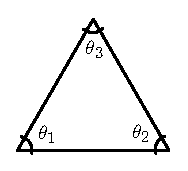
\epsfig{file=chapters/Estimators/gauss_1, height=26mm}
\end{center}
\vspace{-10pt}
\caption{The interior angles of an arbitrary triangle.}
\label{fig:estimators-gauss_1}
\end{figure}

Consider, the interior angles of an arbitrary triangle as shown in Figure~\ref{fig:estimators-gauss_1}. Of course, for a flat triangle, the sum of the interior angles is $\pi$, but for a triangle inscribed on a surface, this is not generally true.  The well-known Gauss-Bonnet theorem tells us that, for any triangle inscribed on a surface, the \emph{integral Gaussian curvature} (also known as the \emph{total curvature}), over the area of the inscribed triangle, is equal to the interior \emph{angle excess}. This can be expressed as:
\begin{equation}
\int K da = (\theta_1 + \theta_2 + \theta_3) - \pi
\end{equation}

In order to extend this idea to polygons, consider an arbitrary inscribed polygon having $n\ge3$ sides, and $n$ interior angles $\phi$, as illustrated in Figure~\ref{fig:estimators-gauss_2}(a). This polygon can be subdivided into $(n-2)$ inscribed triangles as shown in Figure~\ref{fig:estimators-gauss_2}(b). The total curvature over the area of the polygon can be expressed as the sum of total curvatures associated with each of those $(n-2)$ triangles:
\begin{align}
\int K da &= \sum_{T=1}^{n-2} \Bigl( (\theta_1 + \theta_2 + \theta_3) - \pi \Bigr)\\
&= \Biggl( \sum_{T=1}^{n-2} (\theta_1 + \theta_2 + \theta_3) \Biggr) - \Biggl( (n-2)\pi \Biggr)\\
&= \Biggl( \sum_{T=1}^{n-2} (\theta_1 + \theta_2 + \theta_3) \Biggr) + 2\pi - n\pi
\label{eq:estimators-polygon1}
\end{align}

\begin{figure}[!t]
\begin{center}
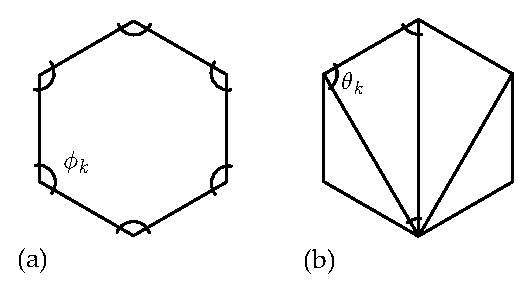
\epsfig{file=chapters/Estimators/gauss_2, height=37mm}
\end{center}
\vspace{-10pt}
\caption{An arbitrary polygon: (a) interior angles, (b) triangulated.}
\label{fig:estimators-gauss_2}
\end{figure}

But, observe that, again with reference to Figure~\ref{fig:estimators-gauss_2}, the sum of all the interior angles $\theta$ in all of the $(n-2)$ triangles is equal to the sum of the $n$ interior angles $\phi$ of the polygon:
\begin{equation}
\sum_{T=1}^{n-2} (\theta_1 + \theta_2 + \theta_3) = \sum_{k=1}^{n} \phi_k
\end{equation}
Substitution into Equation~(\ref{eq:estimators-polygon1}) gives
\begin{equation}
\int K da = \Biggl( \sum_{k=1}^{n} \phi_k \Biggr) + 2\pi - n\pi
\label{eq:estimators-polygon2}
\end{equation}

\begin{figure}[!t]
\begin{center}
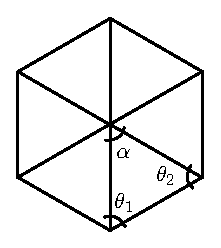
\epsfig{file=chapters/Estimators/gauss_3, height=34mm}
\end{center}
\vspace{-10pt}
\caption{The central angles of an arbitrary triangle umbrella.}
\label{fig:estimators-gauss_3}
\end{figure}

Now consider a triangle mesh digitization of the same (arbitrary) inscribed $n$-sided polygon as illustrated in Figure~\ref{fig:estimators-gauss_3}. Note that we have separately identified a central angle $\alpha$ associated with each of the $n$ triangles. Because these are flat triangles, we have
\begin{equation}
\sum_{T=1}^{n} (\alpha + \theta_1 + \theta_2) = n \pi
\end{equation}
which can be rewritten as
\begin{equation}
\sum_{T=1}^{n} (\theta_1 + \theta_2) = n \pi - \sum \alpha_n
\end{equation}
Note that the left hand side approximates the sum of the inscribed polygon interior angles. Substitution into Equation~(\ref{eq:estimators-polygon2}) gives
\begin{align}
\int K da &\approx \Bigl( n\pi - \sum \alpha_n \Bigr) + 2\pi - n\pi\\
&\approx  2\pi - \sum \alpha_n
\label{eq:estimators-polygon3}
\end{align}

To convert the total (integral) curvature into a curvature value that will be assigned to the central vertex in the triangle umbrella, we need to divide both sides of Equation~(\ref{eq:estimators-polygon3}) by the area over which the integration takes place. Keeping in mind that a curvature value is ultimately assigned at every vertex, and that the overall total area over which we integrate should be equal to the total surface area, we need to somehow apportion the area of each triangle face in the umbrella to each of its three vertices.\\

The required apportioning of area has been done by other authors in various ways; for examples of different area operators used in this context, see \cite{Meyer_2003_DDGO} and \cite{Jagann_2007_3DSMS}. Perhaps the simplest approach is to assign $1/3$ of the area of each face $\cal{A}$ to each of its vertices, and, of course, to sum the contributions from each face at common vertices. Dividing both sides of Equation~(\ref{eq:estimators-polygon3}) by this integration area gives
\begin{equation}
K \approx \frac{(2\pi-\sum{\alpha_n})}{\sum{{\cal A}(f_n) / 3}}= \frac{3(2\pi-\sum{\alpha_n})}{\sum{{\cal A}(f_n)}} = \tilde{K}
\end{equation}
This completes the derivation.\qed
\vspace{20pt}

Referring again to Figure~\ref{fig:estimators-estimators5}, \textbf{mean curvature} at the point $\mathbf{p}_0$ is estimated by
\begin{equation}
\tilde{H}(\mathbf{p}_0) = \frac{3}{4} \biggl( \frac{\sum{\beta_n \, ||e_n||}}{\sum{{\cal A}(f_n)}} \biggr)
\end{equation}
As was the case with the Gaussian curvature estimator, this estimator is also generally valid in the case of any adjacency point count greater than or equal to three. \\

This mean curvature estimator can be derived as follows:\\

\begin{figure}[!t]
\begin{center}
\epsfig{file=chapters/Estimators/estimators2, height=36mm}
\end{center}
\vspace{-10pt}
\caption{Edge smoothed with a cylinder segment.}
\label{fig:estimators-estimators2}
\end{figure}

We begin with the observations that, with any triangle mesh, the curvature of each (flat) face is zero, and the curvature along edges and vertices is undefined because the mesh is not smooth there. So, we consider the effects of smoothing each edge of the mesh using a small arbitrary radius cylinder placed such that mesh faces at the edge are tangent to the cylinder. Figure~\ref{fig:estimators-estimators2} shows an edge corner, in cross-section, smoothed by a circular arc (in bold) with length $l$. Note that, because of the tangential placement of the cylinder, the central angle associated with this smoothing arc is exactly equal to the previously identified dihedral angle $\beta$ between adjacent face normals. By elementary geometry we have
\begin{equation}
l_n = \beta_n r\\
\label{eq:estimators-length}
\end{equation}

Now, since the mean curvature of a cylinder is everywhere $1/2r$ and the area of a smoothed edge is $l$ times the length of the edge, the \emph{integral (total) mean curvature} over a complete triangle umbrella is estimated by
\begin{equation}
\int H da \approx \sum_{k=1}^{n} \Bigl( (1/2r) \, l_n \, ||e_n|| \Bigr)
= \sum_{k=1}^{n} \biggl( \frac{l_n \, ||e_n||}{2r} \biggr)
\end{equation}
Substitution using Equation~(\ref{eq:estimators-length}) gives
\begin{equation}
\int H da \approx \sum_{k=1}^{n} \biggl( \frac{\beta_n r \, ||e_n||}{2r} \biggr)
= \sum_{k=1}^{n} \biggl( \frac{\beta_n \, ||e_n||}{2} \biggr)
\label{eq:estimators-mean1}
\end{equation}

Similarly to the case of Gaussian curvature, we need to divide both sides of Equation~(\ref{eq:estimators-mean1}) by the area over which the integration takes place. As before, we use the simple $1/3$ area operator. However, with mean curvature, edge length also needs to be apportioned between vertices. Consistent with our area operator justification, we assign $1/2$ the length of every edge to its adjacent vertices, which results in
\begin{equation}
H \approx \sum_{k=1}^{n} \Bigl( \frac{\beta_n \, (||e_n||/2)}{2} \Bigr)
\Big/ \sum_{k=1}^{n} {\cal A}(f_n) / 3
= \frac{3}{4} \biggl( \frac{\sum{\beta_n \, ||e_n||}}{\sum{{\cal A}(f_n)}} \biggr)= \tilde{H}
\end{equation}
This completes the derivation.\qed
\vspace{20pt}

Generally, in practical applications, only the point data is given. So, for Gaussian curvature, the angles $\alpha_n$ and the face areas ${\cal A}(f_n)$ need to be calculated. Additionally, for mean curvature, the dihedral angles $\beta_n$ and the edge lengths $e_n$ need to be calculated. With reference to Figure~\ref{fig:estimators-estimators5}, this can be done using vector operations as follows:
\begin{equation}
\alpha_n = \cos^{-1} \Biggl( \frac{(\mathbf{p}_n - \mathbf{p}_0) \cdot (\mathbf{p}_{n+1} - \mathbf{p}_0)}{||(\mathbf{p}_n - \mathbf{p}_0)|| \; ||(\mathbf{p}_{n+1} - \mathbf{p}_0)||}\Biggr)
\end{equation}
\begin{equation}
{\cal A}(f_n) = \frac{||(\mathbf{p}_n - \mathbf{p}_0) \times (\mathbf{p}_{n+1} - \mathbf{p}_0)||}{2}
\end{equation}
\begin{equation}
\beta_n = \cos^{-1} \Biggl( \frac{\bigl((\mathbf{p}_{n-1} - \mathbf{p}_0) \times (\mathbf{p}_{n} - \mathbf{p}_0)\bigr) \cdot \bigr((\mathbf{p}_n - \mathbf{p}_0) \times (\mathbf{p}_{n+1} - \mathbf{p}_0)\bigr)}{||(\mathbf{p}_{n-1} - \mathbf{p}_0) \times (\mathbf{p}_{n} - \mathbf{p}_0)|| \; ||(\mathbf{p}_n - \mathbf{p}_0) \times (\mathbf{p}_{n+1} - \mathbf{p}_0)||}\Biggr)
\end{equation}
\begin{equation}
e_n = ||(\mathbf{p}_n - \mathbf{p}_0)||
\end{equation}

%------------- subsection ----------------
\subsection{Surface Cut}
\label{sec:estimators-cut}

The development of the estimators presented in this section starts with curvature estimation for (discrete) digitized planar curves.\\

\begin{figure}[!t]
\begin{center}
\epsfig{file=chapters/Estimators/estimators3, height=50mm}
\end{center}
\caption{Three surface points: (a) surface cross-section, (b) surface digitization.}
\label{fig:estimators-estimators3}
\end{figure}

Consider a planar curve contained in a surface, along with three points on the curve, as shown in Figure~\ref{fig:estimators-estimators3}(a). Note that the unique plane determined by the three points qualifies as a cutting plane as defined in Section~\ref{sec:curvature-surfaces}. Of course, for example, when working with a digitization that includes these three points, we can only estimate the position of the intermediate connecting points. One very straightforward way to estimate the location of the missing detail is to connect the points with line segments as illustrated in Figure~\ref{fig:estimators-estimators3}(b).\\

Recall, from Section~\ref{sec:curvature-planar-regions}, that (signed) planar line curvature for smooth curves is defined as incremental change in angle divided by incremental change in length. This definition can be applied to a discrete digitization as follows:\\

With reference to Figure~\ref{fig:estimators-estimators3}(b), the curvature at the point $\mathbf{p}_2$ is estimated by
\begin{equation}
\tilde{k}(\mathbf{p}_2) = \frac{\alpha}{(d_1+d_2)/2}
\end{equation}
where $d_1$ and $d_2$ are the distances from $\mathbf{p}_2$ to $\mathbf{p}_1$ and $\mathbf{p}_3$ respectively. Note that he total length $(d_1+d_2)$ has been divided by two because some of this total will be apportioned to curvature estimation at the points $\mathbf{p}_1$ and $\mathbf{p}_3$. The reasoning behind this length operator is similar to the reasoning used for the face area and edge length operators used in Section~\ref{sec:estimators-umbrella}.\\

\begin{figure}[!t]
\begin{center}
\epsfig{file=chapters/Estimators/sweep, height=45mm}
\end{center}
\vspace{-10pt}
\caption{A regular acquisition pattern that results in hexagonal adjacency.}
\label{fig:estimators-sweep}
\end{figure}

To make use of the n-cut mean curvature theory from Section~\ref{sec:curvature-surfaces}, we require digitizations in which equally spaced (by angle) cutting planes can be found. Fortunately, surface digitizations are often acquired mechanically in a regular stepped fashion that results in a symmetry which can be exploited. A common example is illustrated in Figure~\ref{fig:estimators-sweep}, where the acquisition sequence results in a symmetrical hexagonal point adjacency pattern.\\

\begin{figure}[!t]
\begin{center}
\epsfig{file=chapters/Estimators/sweep1, height=45mm}
\end{center}
\vspace{-15pt}
\caption{Estimator point selection for: (a) two cut, (b) three-cut.}
\label{fig:estimators-sweep1}
\end{figure}

Given hexagonal adjacency, both two and three equally spaced cutting planes can be placed by selecting points as illustrated in Figure~\ref{fig:estimators-sweep1}. The curvatures associated with these cutting planes can then be used to estimate surface curvature. For the two-cut mean curvature estimator, we have\\
\begin{equation}
\tilde{H}_{(2\text{-cut})} = \frac{\tilde{\kappa}_1 + \tilde{\kappa}_2}{2}
\end{equation}
and, for the three-cut mean curvature estimator,
\begin{equation}
\tilde{H}_{(3\text{-cut})} = \frac{\tilde{\kappa}_1 + \tilde{\kappa}_2 + \tilde{\kappa}_3}{3}
\end{equation}

\begin{figure}[!t]
\begin{center}
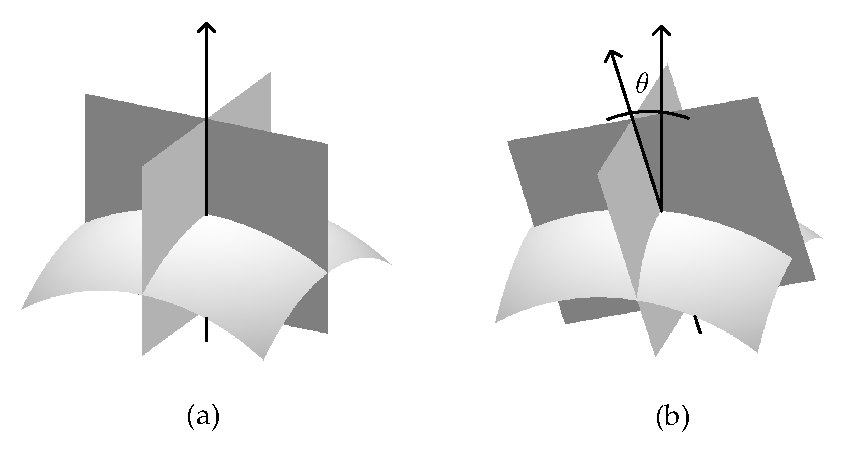
\epsfig{file=chapters/Estimators/estimators4, height=50mm}
\end{center}
\vspace{-15pt}
\caption{Surface cutting planes: (a) aligned with surface normal, (b) misaligned by angle $\theta$.}
\label{fig:estimators-estimators4}
\end{figure}

These estimators have been derived under the assumption that the intersection of the cutting planes aligns with the surface normal as shown, for example, in Figure~\ref{fig:estimators-estimators4}(a). When the cutting planes do not align with the surface normal, a correction, based on Meusnier's theorem (see e.g. \cite{Hermann_2003_MACE}), can be applied, resulting in the following general form for the n-cut estimator:
\begin{equation}
\tilde{H}_{(n\text{-cut})} = \cos \theta \, \Bigl( \frac{\sum \tilde{\kappa}_n}{n} \Bigr)
\label{eq:estimators-mean-cut}
\end{equation}
where $\theta$ is the misalignment angle as shown, for example, in Figure~\ref{fig:estimators-estimators4}(b).\\

As was stated previously, in practical applications, only the point data is given. So, for the surface cut estimator, the angular advance $\alpha$ and the segment lengths $d_n$ need to be calculated. With reference to Figure~\ref{fig:estimators-estimators3}(b), this can be done using vector operations as follows:
\begin{equation}
\alpha = \cos^{-1} \Biggl( \frac{(\mathbf{p}_2 - \mathbf{p}_1) \cdot (\mathbf{p}_3 - \mathbf{p}_2)}{||(\mathbf{p}_2 - \mathbf{p}_1)|| \; ||(\mathbf{p}_3 - \mathbf{p}_2)||} \Biggr)
\end{equation}
\begin{equation}
d_n = ||(\mathbf{p}_{n+1} - \mathbf{p}_n)||
\end{equation}

Additionally, for misaligned cutting planes, $\theta$ needs to be calculated. We present this calculation in several steps, beginning with an estimation of the surface normal vector as a weighted sum (by face area) of the adjacent the face normals. With reference to Figure~\ref{fig:estimators-estimators5}, this sum is\\
\begin{align}
\mathbf{v}_1 &= \sum 2\,{\cal A}(f_n) \; \mathbf{n}_n\\
&= \sum \Bigl( ||(\mathbf{p}_n - \mathbf{p}_0) \times (\mathbf{p}_{n+1} - \mathbf{p}_0)|| \; \bigl((\mathbf{p}_n - \mathbf{p}_0) \times (\mathbf{p}_{n+1} - \mathbf{p}_0)\bigr) \Bigr)
\end{align}\\
Note that, to minimize computation steps, the weighting used is double the face area. This is acceptable because normalization of $\mathbf{v}_1$ occurs later.\\

Next, working with any two of the cutting planes, we calculate a cutting plane intersection vector. With reference to Figure~\ref{fig:estimators-estimators3}, and using additional subscripts $a$ and $b$ to distinguish between the two cutting planes, we calculate\\
\begin{equation}
\mathbf{v}_2 = \Bigl((\mathbf{p}_2 - \mathbf{p}_{a1}) \times (\mathbf{p}_{a3} - \mathbf{p}_2) \Bigr) \times \Bigl( (\mathbf{p}_2 - \mathbf{p}_{b1}) \times (\mathbf{p}_{b3} - \mathbf{p}_2) \Bigr)
\end{equation}\\

Finally, since what's required in Equation~\ref{eq:estimators-mean-cut} is not $\theta$, but rather $\cos \theta$, with reference to Figure~\ref{fig:estimators-estimators4}, we calculate\\
\begin{equation}
\cos \theta = \frac{\mathbf{v}_1 \cdot \mathbf{v}_2}{||\mathbf{v}_1|| \; ||\mathbf{v}_2||}
\end{equation}\\

%===================================================
\section{A Similarity Curvature Estimator}
From Section~\ref{sec:curvature-similarity}, similarity curvature is, by definition,
determined by the principal curvatures. But, because a digitization acquisition pattern
will not, in general, align with the principal curvature directions, we cannot directly
compute the principal curvatures. However, recall, from
Section~\ref{sec:estimators-umbrella} and Section~\ref{sec:estimators-cut}, that we do
already have estimators for mean and Gaussian curvature.\\

Building on this, similarity curvature is estimated using the following process. First the mean and Gaussian curvatures are estimated, then the principal curvatures are calculated from the mean and Gaussian curvatures as follows:
\begin{equation}
\tilde{\kappa}_1 = \tilde{H} + \sqrt{\tilde{H}^2 - \tilde{K}}
\label{eq:invariant-k1}
\end{equation}
\begin{equation}
\tilde{\kappa}_2 = \tilde{H} - \sqrt{\tilde{H}^2 - \tilde{K}}
\label{eq:invariant-k2}
\end{equation}
Finally, the (estimated) similarity curvature is calculated from these principal curvatures
using Definition~\ref{def:curvature-similarity1} and
Definition~\ref{def:curvature-similarity2} as was given in
Section~\ref{sec:curvature-similarity}.\\

Equations~(\ref{eq:invariant-k1}) and (\ref{eq:invariant-k2}) are easily verified. Substitution using Equations~(\ref{eq:curvature-def-mean}) and (\ref{eq:curvature-def-gaussian}) gives
\begin{align}
H + \sqrt{H^2 - K} &= \Bigl(\frac{\kappa_1 + \kappa_2}{2}\Bigr) + \sqrt{\Bigl({\frac{\kappa_1 + \kappa_2}{2}}\Bigr)^2 - \kappa_1 \kappa_2}\\
&= \Bigl(\frac{\kappa_1 + \kappa_2}{2}\Bigr) + \sqrt{\Bigl({\frac{\kappa_1^2 + 2\kappa_1\kappa_2 + \kappa_2^2}{4}}\Bigr) - \Bigl(\frac{4\kappa_1 \kappa_2}{4}\Bigr)}\\
&= \Bigl(\frac{\kappa_1 + \kappa_2}{2}\Bigr) + \sqrt{\Bigl(\frac{\kappa_1^2 - 2\kappa_1\kappa_2 + \kappa_2^2}{4}\Bigr)}\\
&= \Bigl(\frac{\kappa_1 + \kappa_2}{2}\Bigr) + \Bigl(\frac{\kappa_1 - \kappa_2}{2}\Bigr)\\
&= \frac{\kappa_1}{2} + \frac{\kappa_2}{2} + \frac{\kappa_1}{2} - \frac{\kappa_2}{2} = \kappa_1
\end{align}
and
\begin{align}
H - \sqrt{H^2 - K} &= \Bigl(\frac{\kappa_1 + \kappa_2}{2}\Bigr) - \sqrt{\Bigl({\frac{\kappa_1 + \kappa_2}{2}}\Bigr)^2 - \kappa_1 \kappa_2}\\
&= \Bigl(\frac{\kappa_1 + \kappa_2}{2}\Bigr) - \sqrt{\Bigl({\frac{\kappa_1^2 + 2\kappa_1\kappa_2 + \kappa_2^2}{4}}\Bigr) - \Bigl(\frac{4\kappa_1 \kappa_2}{4}\Bigr)}\\
&= \Bigl(\frac{\kappa_1 + \kappa_2}{2}\Bigr) - \sqrt{\Bigl(\frac{\kappa_1^2 - 2\kappa_1\kappa_2 + \kappa_2^2}{4}\Bigr)}\\
&= \Bigl(\frac{\kappa_1 + \kappa_2}{2}\Bigr) - \Bigl(\frac{\kappa_1 - \kappa_2}{2}\Bigr)\\
&= \frac{\kappa_1}{2} + \frac{\kappa_2}{2} - \frac{\kappa_1}{2} + \frac{\kappa_2}{2} = \kappa_2
\end{align}

Finally, to estimate similarity curvature, the principal curvature estimates $\tilde{\kappa}_1$ and $\tilde{\kappa}_2$ can be plugged directly into Equation~(\ref{eq:similarity-curvature}).\\

%---------------- section ----------------
\section{Estimators Summary}
The estimators presented in this chapter can be divided into four groups:\\
1) n-neighborhood triangle umbrella Gaussian,\\
2) n-neighborhood triangle umbrella mean,\\
3) n-cut mean, with or without compensation,\\
4) similarity curvature - using both the Gaussian and mean curvatures.\\

In practice, the application of these estimators will depend on identifying point 
neighborhoods and, for the n-cut mean estimator, identifying points which give equally 
spaced cutting planes. We note that the n-cut uncompensated mean estimator calculation has 
the least number of operations and would thus have the fastest computational execution time.\\


